\documentclass[a4paper]{article}
\usepackage[UTF8]{ctex}
\usepackage{geometry}
\usepackage{graphicx}
\usepackage{url}
\usepackage{multirow}
\usepackage{array}
\usepackage{booktabs}
\usepackage{url}
\usepackage{enumitem}
\usepackage{graphicx}
\usepackage{float}
\usepackage{amssymb}
\usepackage{amsmath}
\usepackage{subfig}
\usepackage{longtable}

\geometry{a4paper, scale=0.78}

\title{Math Basis 02}
\author{Chen Gong}
\date{19 October 2019}

\begin{document}

\maketitle
本节的主要目的是从概率的角度来分析高斯分布,包括马氏距离和高斯分布的几何表示,以及高斯分布的局限性和解决的方法等等。对于多变量的高斯分布$X\sim \mathcal{N}(\mu,\Sigma)$,概率密度函数为:
\begin{equation}
    p(X)=\frac{1}{\sqrt{2\pi}^{\frac{p}{2}}|\Sigma|^{\frac{1}{2}}}exp\left\{ -\frac{1}{2}(X-\mu)^T\Sigma^{-1}(X-\mu) \right\}
\end{equation}
其中,$X\in\mathbb{R}^p$,
\begin{equation}
    X=
    \begin{pmatrix}
        x_1 \\
        x_2 \\
        \vdots \\
        x_p
    \end{pmatrix} \qquad \qquad
    \Sigma = 
    \begin{pmatrix}
        \sigma_{11} & \sigma_{12} & \cdots & \sigma_{1p} \\
        \sigma_{21} & \sigma_{22} & \cdots & \sigma_{2p} \\
        \vdots      & \vdots      & \ddots & \vdots      \\
        \sigma_{p1} & \sigma_{p2} & \cdots & \sigma_{pp}
        \end{pmatrix}
\end{equation}
其中,$\Sigma$一般为正定矩阵或者为半正定矩阵。

\section{什么是马氏距离}
在高斯分布中,$(X-\mu)^T\Sigma^{-1}(X-\mu)$的计算结果是一个数,这个数被称为马氏距离。设$z_1=(z_{11}, z_{12})^T$,$z_1=(z_{21}, z_{22})^T$。那么$z_1$和$z_2$之间的马氏距离为,
\begin{equation}
    (z_1-z_2)^T\Sigma^{-1}(z_1-z_2)=
    \begin{pmatrix}
        z_{11}-z_{12} & z_{21}-z_{22}
    \end{pmatrix}
    \Sigma^{-1}
    \begin{pmatrix}
        z_{11}-z_{12} \\
        z_{21}-z_{22}
    \end{pmatrix}
\end{equation}

显然,当$\Sigma^{-1}=I$时,马氏距离等于欧式距离$ (z_1-z_2)^T\Sigma^{-1}(z_1-z_2)=(z_{11}-z_{12})^2+(z_{21}-z_{22})^2$。

\section{对$(X-\mu)^T\Sigma^{-1}(X-\mu)$的值进行推导}
由于$\Sigma$为实对称矩阵,那么可以对$\Sigma$进行特征分解,那么有$\Sigma = U\Lambda U^T$,并且$UU^T=U^TU=I$,所以$U^{-1}=U^T$,$\Lambda=diag(\lambda_i)\quad(i=1,2,\cdots,N)$,并且$U=(U_1,U_2,\cdots,U_p)_{p\times p}$。

\begin{align}
    \Sigma = & U\Lambda U^T \\
    = & (U_1,U_2,\cdots,U_p)
    \begin{pmatrix}
        \lambda_1 & & & \\
        & \lambda_2 & & \\
        & & \ddots & \\
        & & & \lambda_p \\
    \end{pmatrix}
    \begin{pmatrix}
        U_1^T  \\
        U_2^T  \\
        \vdots \\
        U_p^T  \\
    \end{pmatrix} \\
     = & (U_1\lambda_1,U_2\lambda_2,\cdots,U_p\lambda_p)
     \begin{pmatrix}
        U_1^T  \\
        U_2^T  \\
        \vdots \\
        U_p^T  \\
    \end{pmatrix} \\
    = & \sum_{i=1}^{p}U_i\lambda_i U_i^T
\end{align}

而$\Sigma^{-1}$的求解过程如下所示:

\begin{equation}
    \Sigma^{-1} = (U \Lambda U^T)^{-1} = (U^T)^{-1} \Lambda^{-1} U^{-1} = U \Lambda^{-1} U^T
\end{equation}

代入可以解得:
\begin{equation}
    \Sigma^{-1} = \sum_{i=1}^{p}U_i\frac{1}{\lambda_i} U_i^T
\end{equation}

那么,
\begin{align}
    (X-\mu)^T\Sigma^{-1}(X-\mu) = & (X-\mu)^T\sum_{i=1}^{p}U_i\frac{1}{\lambda_i} U_i^T(X-\mu) \\
    = & \sum_{i=1}^{p} (X-\mu)^TU_i\frac{1}{\lambda_i} U_i^T(X-\mu)
\end{align}

令$y_i=(X-\mu)^TU_i$,这是一个典型的投影算法,其中$U_i$是特征值为$\lambda_i$的特征向量,那么
\begin{equation}
    (X-\mu)^T\Sigma^{-1}(X-\mu) = \sum_{i=1}^{p} y_i\frac{1}{\lambda_i} y_i^T
\end{equation}

\section{高斯分布的几何意义}
如何令$p=2$,则有$\Delta = \frac{y_1^2}{\lambda_1} + \frac{y_2^2}{\lambda_2} $,这实际上就是一个椭圆,如果$\Delta$取不同的值,就会像等高线一样,一圈圈的环绕。而$y$实际上相当于先平移后投影(旋转),那么最终的效果图画表示为:
\begin{figure}[H]
    \centering
    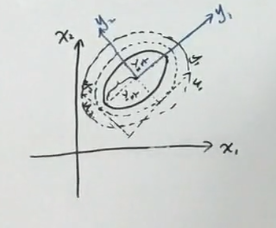
\includegraphics[width=.5\textwidth]{20191019203302.png}
    \caption{二维高斯分布的可视化表示图}
    \label{fig:my_label_1}
\end{figure}

这里使用到了投影算子。

\section{高斯分布中遇到的困难}
\subsection{维度灾难(curse of dimension)}
由于$\Sigma$是一个$p\times p$的矩阵,矩阵中一共有$\frac{p(p+1)}{2}$个参数,算法的复杂度为$O(p^2)$。一旦输入维度过大,这个矩阵的计算会变得很复杂。所以,在某些时候,将$\Sigma$矩阵简化成对角矩阵将算法复杂度降低到$O(p)$。进一步简化,可以令$\lambda_1=\lambda_2=\cdots=\lambda_p$。这时,高斯分布的可视化表示即为一个中心在原点的同心圆。这样的高斯分布,被我们称为“各向同性”的高斯分布。

\subsection{高斯分布的表达的局限性}
很多时候,高斯分布的表达有局限性,这时,学者提出了混合高斯模型(GMM)来拟合现实情况中复杂多样的分布。具体有关于混合高斯模型(GMM)的内容将在后续部分进行详细解释,
\end{document}